\section{Modelo de negocio}
\subsection{Esquema de modelo de negocio (CANVAS)}

A continuación se profundiza en cada uno de los aspectos presentados en el modelo canvas de la Figura \ref{ModeloCanva}


\vspace{2mm}
        \begin{minipage}{0.9\textwidth}
        \centering
        \captionof{figure}[{Modelo de Negocio}]{ Modelo de Negocio.}
        \label{ModeloCanva}
         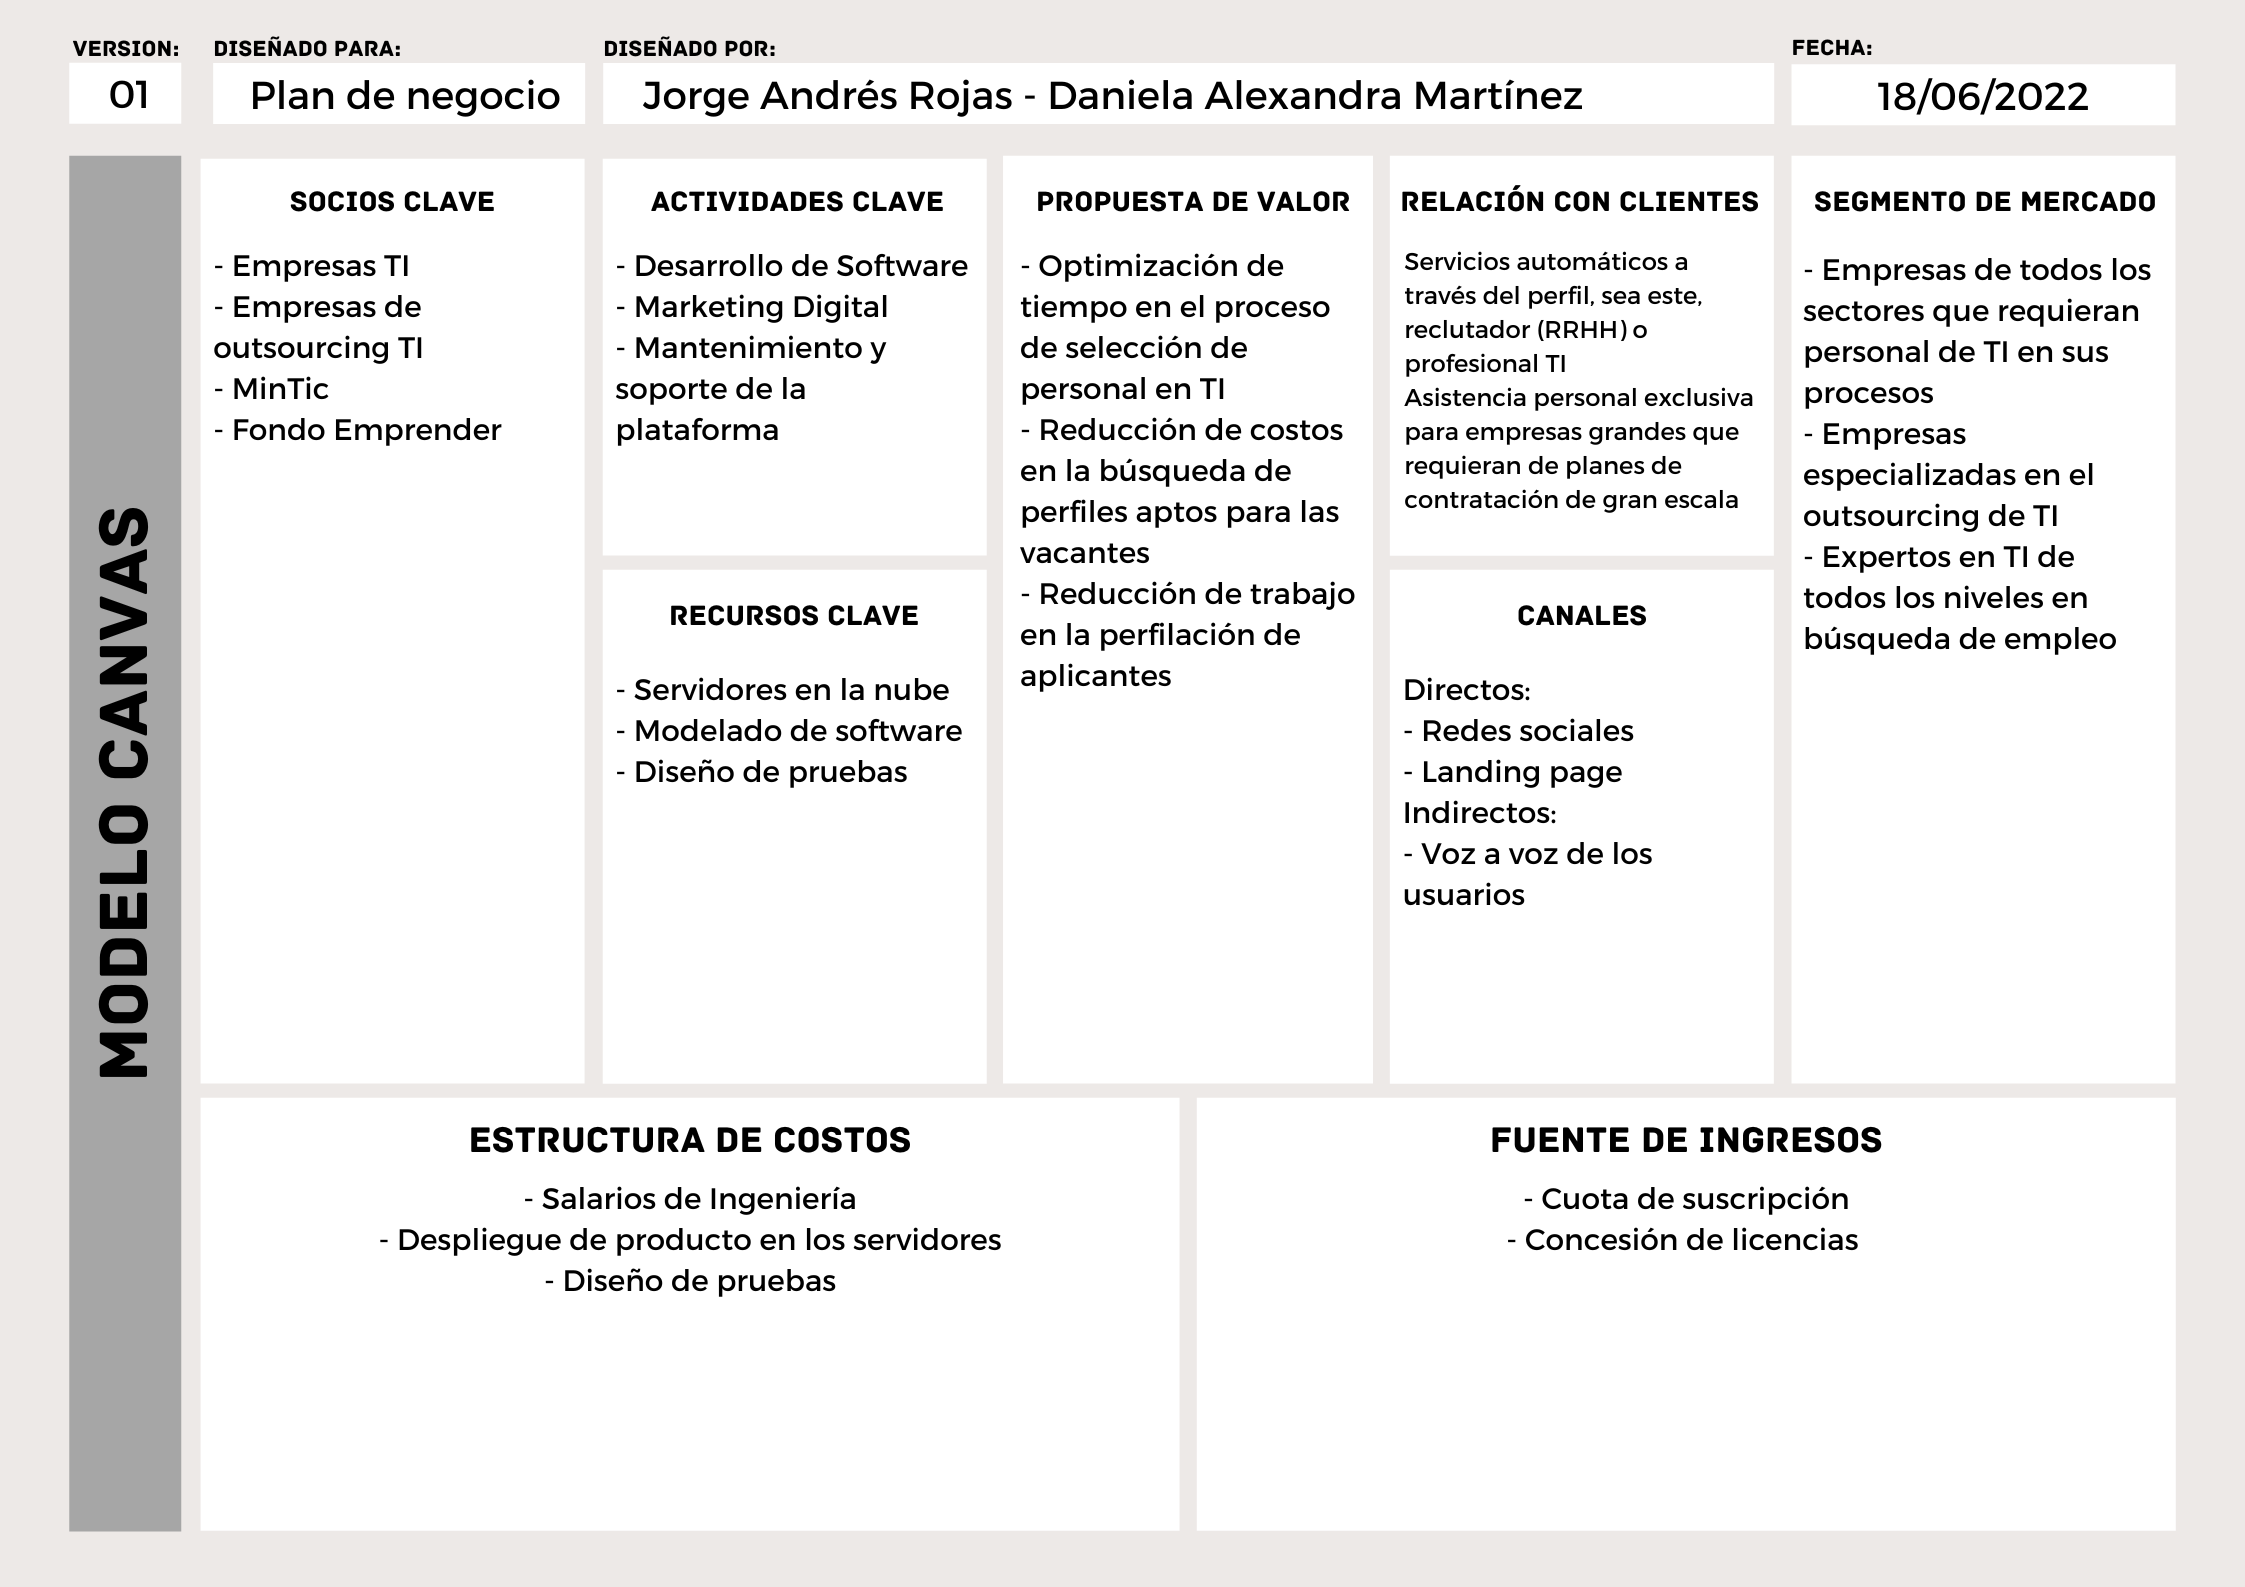
\includegraphics[width=\textwidth]{Images/modelocanva}
          %esto es lo nuevo que agregue
        \fnote{Nota. \textup{Fuente: Autores.}}
\end{minipage}
        
\subsubsection*{Segmento de mercado (SM)}


Este modulo abarca los clientes a los que va dirigido el producto o servicio. Los grupos de clientes pertenecen a segmentos de acuerdo a las necesidades que requieren. Nuestro segmento corresponde a empresas dedicadas a la contratación y uso de personal TI. 

\subsubsection*{Propuesta de valor (PV)}

En esta sección se da conocer qué productos y servicios suplen la necesidad de nuestro segmento de clientes. Es por medio de este factor que el cliente se inclinara a escoger una u otra empresa. La propuesta de valor que ofrecemos es una optimización de procesos de contratación en la empresas TI de la ciudad de Bogotá por medio de gamificación, el uso de esta técnica marca una diferencia tanto en los aspirantes al encontrar mas motivador el ingreso a un posible puesto de trabajo como a la empresa cliente que reducirá sus tiempos y costos en la búsqueda de talento humano.

\subsubsection*{Canales de distribución (CD)}

Los canales son el medio por el cual se comparte la propuesta de valor a los potenciales clientes. Para ello se dispone de la landing page además de canales de atención como lo son redes sociales y correo electrónico. También se espera contar con el canal voz a voz de los usuarios de nuestro producto.

\subsubsection*{Relación con clientes (RCl)}

Este modulo mencionan las diferentes formas en las que la empresa se relaciona con el segmento de mercado. Según el tipo de relación que se maneje esta repercutirá en la experiencia global del cliente. Por lo que se espera en primer lugar una relación de atomización, en el sentido de que el cliente hace uso de la plataforma de manera autónoma para acceder al servicio.

\subsubsection*{Fuentes de ingresos (FI)}

En lo respectivo al flujo de caja esta descrito en el modulo de fuentes de ingresos, aquí es importante cuestionar el valor que los clientes realmente están dispuestos a pagar por el servicio y como desean realizar el pago. Para esto se proponen dos métodos de ingreso, el primero enfocado a cuotas de suscripción por distintos periodos de tiempo, asociado sobretodo a proyectos de corto plazo y el segundo es la concesión de licencias para empresas con un portafolio de proyectos mas amplio.

\subsubsection*{Recursos clave (RC)}

Esta sección describe los insumos necesarios para que el modelo de negocio funcione. Aquí se encuentran las instalaciones físicas, como recursos económicos y/o el capital humano. En nuestro modelo de negocio se destacan los servicios cloud que permitirán poner el servicio (plataforma web) a disposición del cliente; el capital humano que llevara a cabo la implementación de la idea ; Y una arquitectura escalable que garantiza el funcionamiento y mantenimiento a futuro de la plataforma.

\subsubsection*{Actividades clave (AC)}

Las acciones de mayor prioridad para hacer funcionar el modelo de negocio son las actividades claves. La manera en que las implementemos sera crucial para tener éxito. Para nuestro caso están el desarrollo de la plataforma web, el mantenimiento y soporte constante. Como también el marketing como medio para llegar a las personas y entrar al mercado.

\subsubsection*{Socios clave (AsC)}

En este modulo se describirán las redes de proveedores y socios que contribuyen al funcionamiento de un modelo de negocio. Para nuestro plan de negocio serán las empresas TI, empresas de outsourcing en TI, MinTic y Fondo Emprender.

\subsubsection*{Estructura de costos (EC)}

En esta sección se describen todos los costos que implican la puesta en marcha del modelo de negocio. Se debe tener en cuenta el coste de las actividades, recursos claves o incluso el mantenimiento de las relaciones con los clientes. Se espera que la estructura de costos se conforme en gran medida por los servicios de hosting en la nube de la plataforma, los salarios de los empleados y los servicios de marketing.
